\documentclass[11pt,a4paper]{article}
    \usepackage[margin=2.5cm]{geometry}
    \usepackage{enumitem}
    \usepackage{hyperref}
    \usepackage{tikz}
    \usetikzlibrary{arrows.meta,positioning,shapes.geometric}
    \title{RNA and Transcriptomics Tools}
\author{Jordi Vill\`a-Freixa \texttt{<jordi.villa@uvic.cat>}}
    \date{\today}

    \tikzset{
      methodbox/.style={
        rounded corners=6pt,
        draw=blue!50!black,
        line width=0.9pt,
        fill=blue!6,
        minimum width=13cm,
        text width=11.8cm,
        align=left,
        inner sep=8pt
      }
    }

    \begin{document}
    \maketitle

    \section*{Scope}
    This folder focuses on introductory transcriptomics workflows, especially count-based differential expression analysis, annotation lookups, and simple GEO data exploration.

    \section*{Material in this folder}
    \begin{itemize}[leftmargin=*]
\item \texttt{DifferentialExpressionExample.ipynb}
\item \texttt{ENSMBLE2GENENAME.ipynb}
\item \texttt{SimpleAnalysisGEO.ipynb}
\item \texttt{DSeq2.R}
\item \texttt{plot\_minimal\_pydeseq2\_pipeline.py}
\item \texttt{plot\_step\_by\_step.py}
    \end{itemize}

    \section*{Method summary}
    \begin{itemize}[leftmargin=*]
\item \textbf{Differential expression with DESeq2-style models}. The R and Python materials work with count matrices, sample metadata, normalization, dispersion estimation, and hypothesis testing for differential expression.
\item \textbf{PyDESeq2 workflows}. The Python scripts mirror the DESeq2 statistical workflow through count filtering, model fitting, and result extraction.
\item \textbf{Gene annotation lookup}. The ENSMBL notebook maps gene identifiers to names to support downstream interpretation.
\item \textbf{Exploratory GEO analysis}. The notebooks load expression tables and metadata to perform basic transcriptomics data inspection.
    \end{itemize}

    \section*{Method scheme}
    Figure~\ref{fig:summary} is drawn directly in LaTeX with TikZ. It is a compact conceptual map of the main workflows discussed in this folder.

    \begin{figure}[ht]
    \centering
    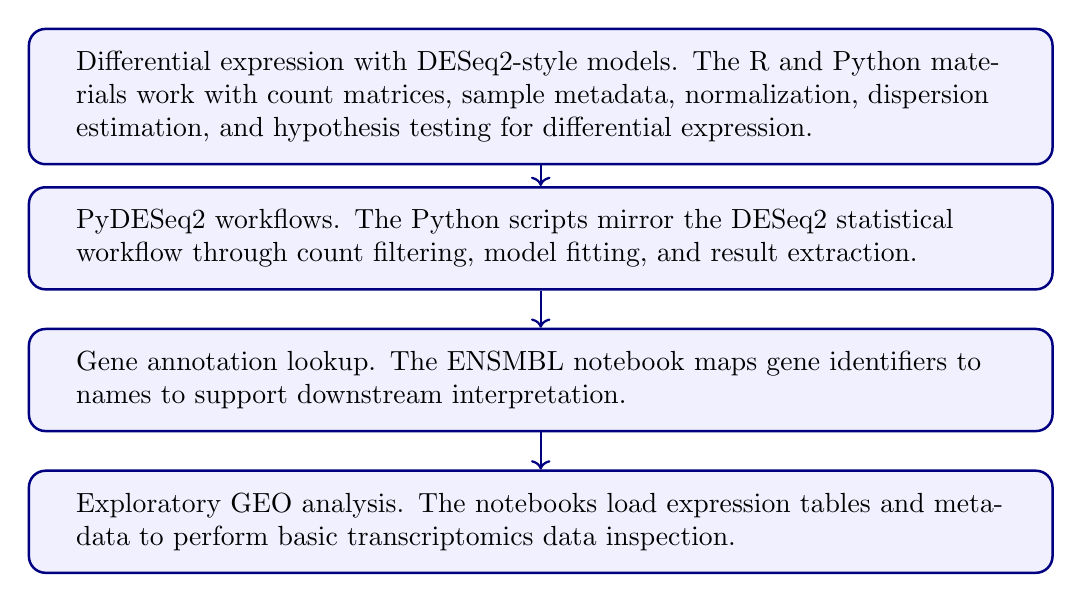
\begin{tikzpicture}[x=1cm,y=1cm]
    \node[methodbox] (m0) at (0,0.0) {Differential expression with DESeq2-style models. The R and Python materials work with count matrices, sample metadata, normalization, dispersion estimation, and hypothesis testing for differential expression.};
    \node[methodbox] (m1) at (0,-1.8) {PyDESeq2 workflows. The Python scripts mirror the DESeq2 statistical workflow through count filtering, model fitting, and result extraction.};
    \node[methodbox] (m2) at (0,-3.6) {Gene annotation lookup. The ENSMBL notebook maps gene identifiers to names to support downstream interpretation.};
    \node[methodbox] (m3) at (0,-5.4) {Exploratory GEO analysis. The notebooks load expression tables and metadata to perform basic transcriptomics data inspection.};
    \draw[->, thick, color=blue!50!black] (m0.south) -- (m1.north);
    \draw[->, thick, color=blue!50!black] (m1.south) -- (m2.north);
    \draw[->, thick, color=blue!50!black] (m2.south) -- (m3.north);
    \end{tikzpicture}
    \caption{Conceptual scheme for the methods in the RNATools folder.}
    \label{fig:summary}
    \end{figure}

    
\section*{Disclaimer}
These documents were generated with the assistance of ChatGPT 5.4. The material has been reviewed by the author before inclusion in this repository, but it is not free from possible errors.

\end{document}